% ------ headers globales -------------
%11pt, , twoside
\documentclass[a4paper]{article}
\usepackage{caratula}
\usepackage[spanish]{babel}
\usepackage[utf8]{inputenc}
\usepackage{amsmath}
\usepackage{float}
\usepackage{url}
%\usepackage[normalem]{ulem}

\begin{document}{}

% -------------------------------------
% -- Carátula --
\newpage{\pagestyle{empty}% parametros para la caratula (caratula.sty)


\materia{Teoría de las Comunicaciones}
\titulo{Trabajo Práctico 3}
\subtitulo{Capa de Transporte: Programación de protocolos end-to-end}
\fecha{14 de Noviembre de 2014}
\integrante{Juan Manuel Tastzian}{39/10}{jm@tast.com.ar}
\integrante{Lucas Tolchinsky}{591/07}{lucas.tolchinsky@gmail.com}
\integrante{Nicolás Vallejo}{500/10}{nico\_pr08@hotmail.com}

\maketitle
}

\setcounter{page}{1}

%-- Indice --
\newpage{\pagestyle{empty}\tableofcontents\cleardoublepage}


\section{Introducción}

\subsection{Retransmission Timeout (RTO)}

El \textit{timeout de retransmisión} es un valor utilizado en protocolos como
\textbf{TCP} que sirve para \textit{asegurarse la entrega} de un paquete al
recipiente, a pesar de la ausencia de todo \textit{feedback} de su parte.\\
\\
\indent Para computar el \textbf{RTO} actual, el emisor del paquete mantiene dos
variables
de estado: \textbf{SRTT} (\textit{smoothed round-trip time}) y \textbf{RTTVAR}
(\textit{round-trip time variation}).\\
\\
\indent Cualquier implementación debe manejar el/los timer(s) de retransmisión
de forma tal que \textit{un segmento \textbf{nunca} es retransmitido demasiado
temprano} (es decir, en menos de un RTO luego de la transmisión del segmento
anterior).\\
\\
\indent A continuación, dejamos el algoritmo \textbf{recomendado} en el
\textbf{RFC 6298} para el manejo del timer de retransmisión:
\begin{enumerate}
 \item Cada vez que se envía un paquete con datos (incluyendo una
	retransmisión), si el timer no está corriendo, se inicia el mismo para
	que expire luego de \textit{RTO} segundos (para el valor actual de
	\textit{RTO}).
 \item Cuando se hizo \textit{ACK} de todos los datos, se apaga el timer de
	retransmisión.
 \item Cuando se recibe un \textit{ACK} que confirma nuevos datos, se reinicia
	el timer de retransmisión para que expire luego de \textit{RTO}
	segundos (para el valor actual de \textit{RTO}).
\end{enumerate}
Cuando expira el timer de retransmisión, hacer lo siguiente:
\begin{enumerate}
 \setcounter{enumi}{3}
 \item Retransmitir el segmento más viejo que no haya sido confirmado
	por el receptor de TCP.
 \item El emisor debe setear \textbf{RTO $\leftarrow$ RTO * 2} (``hacer
	\textit{back off} del timer"). Como valor para acotar superiormente
	esta operación, se puede usar el valor de 60 segundos.
 \item Comenzar el timer de retransmisión para que expire luego de \textit{RTO}
	segundos (para el valor de \textit{RTO} conseguido luego de hacer la
	operación de duplicación en el ítem número 5).
 \item Si expira el timer esperando el \textit{ACK} de un segmento \textit{SYN}
	y la implementación está usando un \textit{RTO} menor a 3 segundos, el
	\textit{RTO} debe ser re-inicializado a 3 segundos cuando comienza la
	transmisión de datos (es decir, luego de finalizar el three-way handshake).
\end{enumerate}

\newpage

\section{Desarrollo}

Para realizar las capturas de paquetes necesarias para la confección de este trabajo práctico se implementó una herramienta en python utilizando las bibliotecas de scapy.En el archivo \textit{sniffer.py} se encontrará el código fuente de la \textit{tool}. Consideramos oportuno mencionar que nuestra herramienta captura, en modo promiscuo, todos los paquetes que puede de la red local para luego volcarlo en un archivo con extensión \textit{.pcap}, soportado por aplicaciones como Wireshark.\newline

Si bien es cierto que scapy nos provee la funcionalidad suficiente como para simplemente capturar los ARP necesarios, nos pareció lógico que la herramienta capturase todo lo que pudiese, puesto que filtrar los datos con el Wireshark es bastante fácil de hacer.\newline

En el archivo \textit{helpers.py} se podrá encontrar todas las funciones encargadas del cálculo de las entropías de las fuentes origen y destino. Con ayuda de un intérprete de Python como \textit{iPython} dichas funciones son fácilmente aplicables.\newline

Sobre el cálculo de la entropía queríamos comentar ciertas cuestiones. En primer lugar, que en vez de la probabilidad de aparición de cada IP utilizaremos la frecuencia de aparición de dicha dirección como fuente o destino de toda la captura dependiendo del caso. En segundo lugar, que calculamos para cada caso la frecuencia de aparición de todas las IP's tanto origenes como destino y luego realizamos el cálculo de la entropía. Notar que si una IP sólo aparece como fuente no impactará en el cálculo de la entropía para la fuente de IP's destino y viceversa, puesto que su frecuencia de aparición en dicha fuentes será igual a cero.\newline

Además, se implementaron dos scripts en Python que se encargan de, dado un archivo .pcap, exportar a formatos .tgf (Trivial Graph Format) y .dot respectivamente, que nos ayudaran para la armado de los grafos.\newline

Como hemos mencionado anteriormente, nuestro capturador no captura únicamente paquetes ARP who-has. Para obtener solamente esos paquetes, al archivo .pcap exportado por el script lo filtramos con la guarda \textit {arp.opcode= = 1 \&\&  !arp.isgratuitous} con Wireshark y luego lo exportamos a otro archivo .pcap que sólo contendrá los paquetes ARP who-has no gratuitos (los paquetes gratuitos son aquellos que algún host envía con su dirección para que los demás host de la red puedan actualizar su tabla de direcciones).\newline

\newpage

\section{Experimentación}

\subsection{Caso de estudio: Red laboral}

Antes de analizar la captura sosteníamos como hipótesis que la topología de los mensajes ``tendría forma de árbol'' con el router en su raíz y tantas hojas como hosts dentro de la red, con poco o nada de interacción entre ellos.\newline

También suponíamos que la mayoría de las redes \textit{subneteadas} con un router tendrían necesariamente esta forma.\newline

En este caso estudiamos la red de una oficina con alrededor de 40 computadoras y teléfonos celulares.\newline

La captura duró alrededor de seis horas con más de 90000 mensajes ARP who-has. Con este volumen de datos fue necesario seccionar el análisis bajo diferentes criterios, como la cantidad de mensajes o una cantidad mínima de mensajes entre nodos.\newline

Los grafos presentados a continuación muestran direcciones IP como nodos unidos por un eje si el nodo origen realizó un broadcast ARP who-has buscando al nodo destino.\newline

Para empezar, mostramos los primeros 10 mil requests entre los nodos que se enviaron diez o más mensajes. Elegimos esta parte de la muestra tras haber visto que graficar más nodos agrega poca información nueva respecto de los nodos más relevantes.\newline

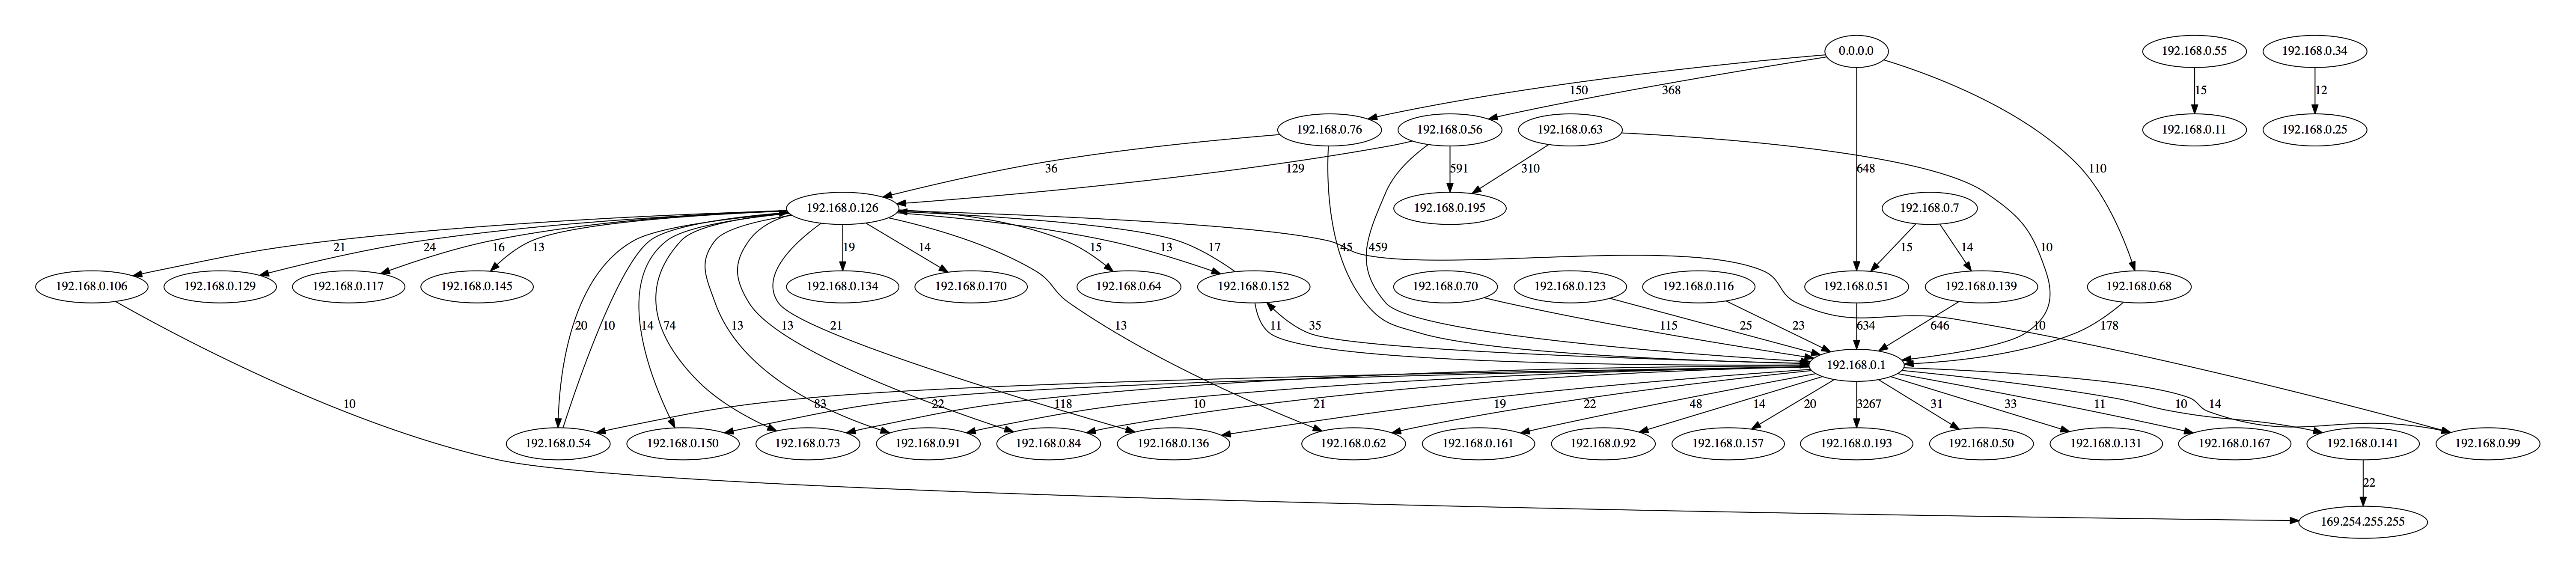
\includegraphics[scale=0.25,angle=90]{graphics/t-work-10000c-10w.png}

A primera vista notamos que hay ciertos nodos que resaltan sobre los demás como el 192.168.0.1 (router), o 192.168.0.126. Si bien la estructura de este digrafo no es un árbol, se nota que hay cierta jerarquía.\newline

Un nodo interesante que resalta es el 169.254.255.255, porque es la única IP no privada que aparece en la red. Analizando este caso en particular, vemos que siempre es buscado por nodos de la red (y éste nunca busca a nadie), lo que nos hace suponer que puede tratarse de un servicio, como un servidor de DNS.\newline

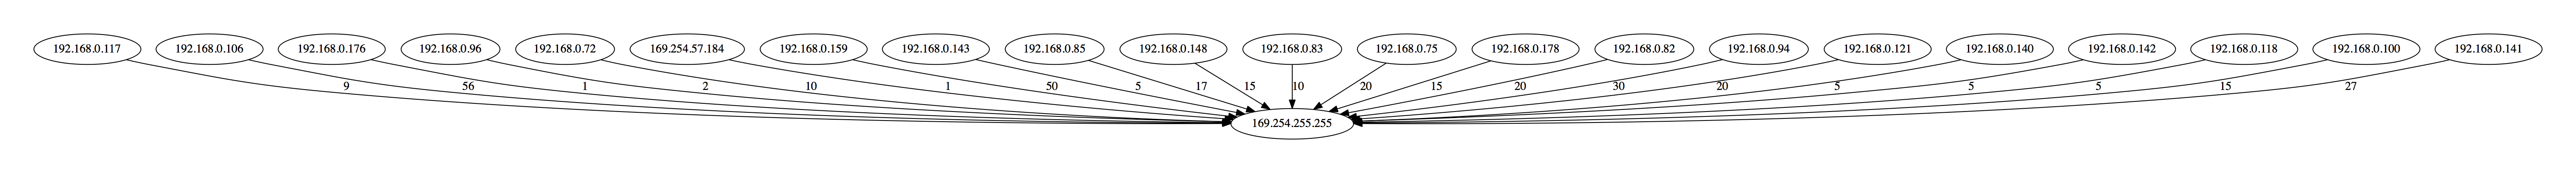
\includegraphics[scale=0.25,clip=true,trim=850 0 870 0]{graphics/t-work-ip-169-254-255-255.png}

Investigando el resto de la captura, notamos que los demás paquetes que recibe son del protocolo NetBIOS Name Service, con lo que podemos afirmar que en este nodo funciona un NetBIOS Server.\newline

Para poder reconocer mejor cuáles son los nodos más importantes de la red veamos el siguiente grafo, donde se estudia toda la muestra pero sólo nos quedamos con aquellos nodos que compartieron más de mil mensajes.\newline

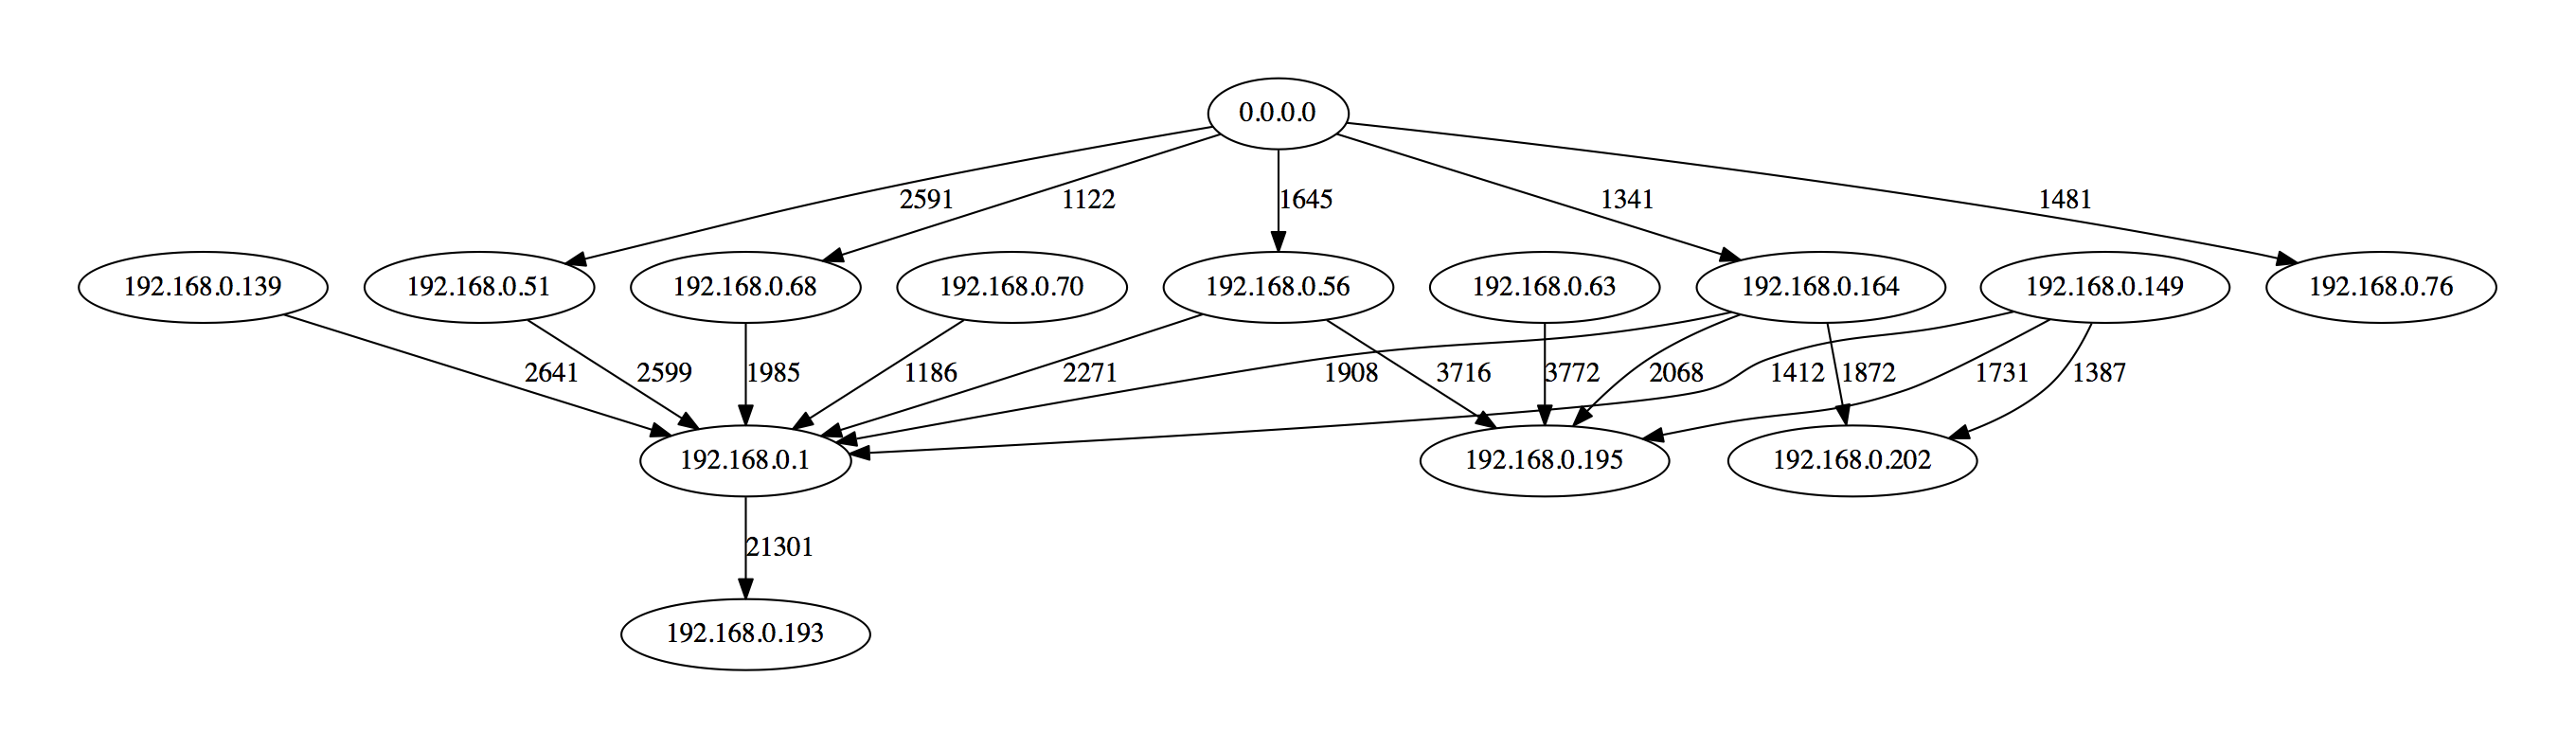
\includegraphics[scale=0.30]{graphics/t-work-all-1000w.png}

Viendo los mensajes ARP de esta manera podemos notar varias cosas. Por un lado que tiene forma de árbol, pero el nodo raíz no es el router, como suponíamos originalmente. Vemos que hay muchos requests ARP que tienen origen en el 0.0.0.0 y como destino diversos nodos de la red, pero ésta no es una IP del rango privado.\newline

Este primer hecho nos llevó a conocer que un ARP con origen 0.0.0.0 es parte de una técnica para detectar direcciones IP duplicadas dentro de una red. En este caso, se estaba queriendo detectar si las direcciones terminadas en 51, 56, 68, 76 ó 164 estaban duplicadas.\newline

\newpage

También nos pareció relevante analizar el router en particular.\newline

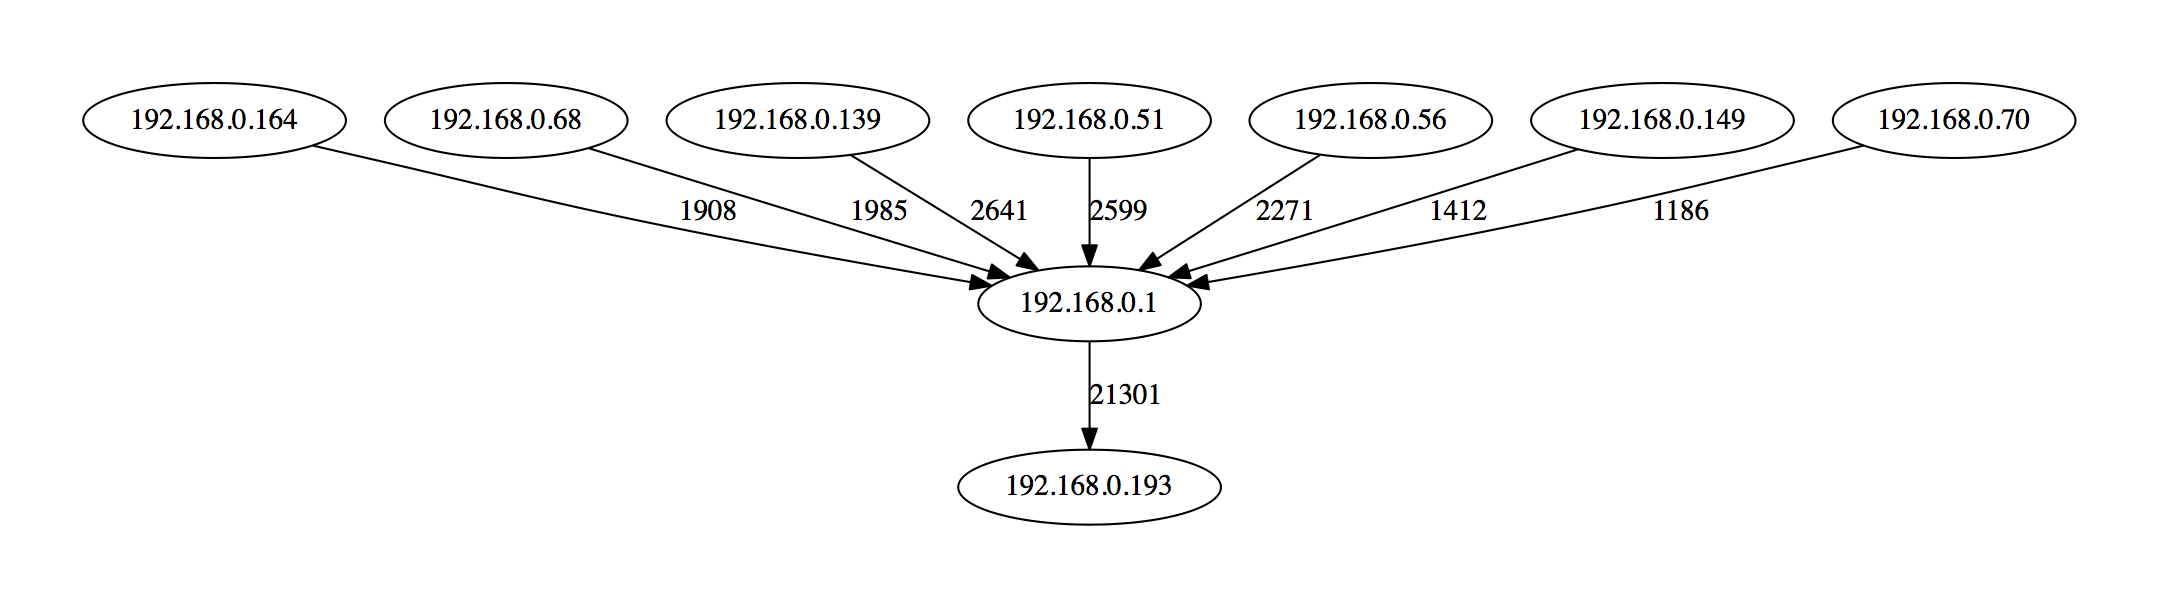
\includegraphics[scale=0.3]{graphics/t-work-router-1000w.png}

Vemos que resulta interesante la gran cantidad de veces que se solicita la IP 192.168.0.193. Para saber más sobre lo que podría estar sucediendo con ese host, revisamos el resto de la captura pero encontramos que no había ningún paquete con esa dirección origen ni destino.\newline

Por esto creemos que podría tratarse de un nodo mal configurado, buscando una IP que ya no existe en la red, lo cual parece en consonancia con la gran cantidad de pedidos ARP que el router le hace.\newline

Finalmente, calculamos la entropía de las fuentes origen y destino: 3.44356252078915 y 4.652923252101102, respectivamente.\newline


\newpage

\section{Conclusiones}


	%-- Bibliografia --
	%\subsection{Bibliografía}
	%\begin{thebibliography}{99}
%		\bibitem{lib:brassard} G. Brassard, P. Bratley, \textit{Fundamental of Algorithmics}, Prentice Hall,  1996, Chapter 6.2, \enquote{General characteristics of greedy algoritmhs}, Chapter 9.6, \enquote{Backtracking}, 
%		\bibitem{lib:cormen} Cormen, Leiserson, Rivest \textit{Introduction to Algorithms}, 2001, Chapter 16 \enquote{Greedy Algorithms}.
%		\bibitem{stl:stl} \texttt{http://www.cplusplus.com/reference/stl/}
		%\bibitem{stl:set} \texttt{http://www.cplusplus.com/reference%/set/set/}
%		\bibitem{stl:vector} \texttt{http://www.cplusplus.com/reference/vector/vector/}
%		\bibitem{stl:pqueue} \texttt{http://www.cplusplus.com/reference/queue/priority\_queue/}
%		\bibitem{wiki:greedy} \texttt{http://en.wikipedia.org/wiki/Greedy\_algorithm\#Specifics}
%		\bibitem{wiki:back} \texttt{http://en.wikipedia.org/wiki/Backtracking\#Usage\_considerations}
%	\end{thebibliography}
	


\end{document}